\section{Unit Tests} \label{sec:Testing-UnitTesting}
The implementations containing specific data handling procedures are the F\# modules, the C\# classes responsible for interaction with the model as well as the classes for communicating with the impact computation module.

These can be visualised in figure \ref{fig:TestingGroups}, showing the units and components which are going to be tested with unit tests. In this figure the light blue squares (as indicated by the legend in the bottom of the figure) are data classes, and therefore not the main focus for testing. 
However, they depend on the class called \texttt{TimestampedList}, which contains functionality regarding the use of lists with timestamped data points, making it important to test.

\begin{figure}[H]
    \centering
    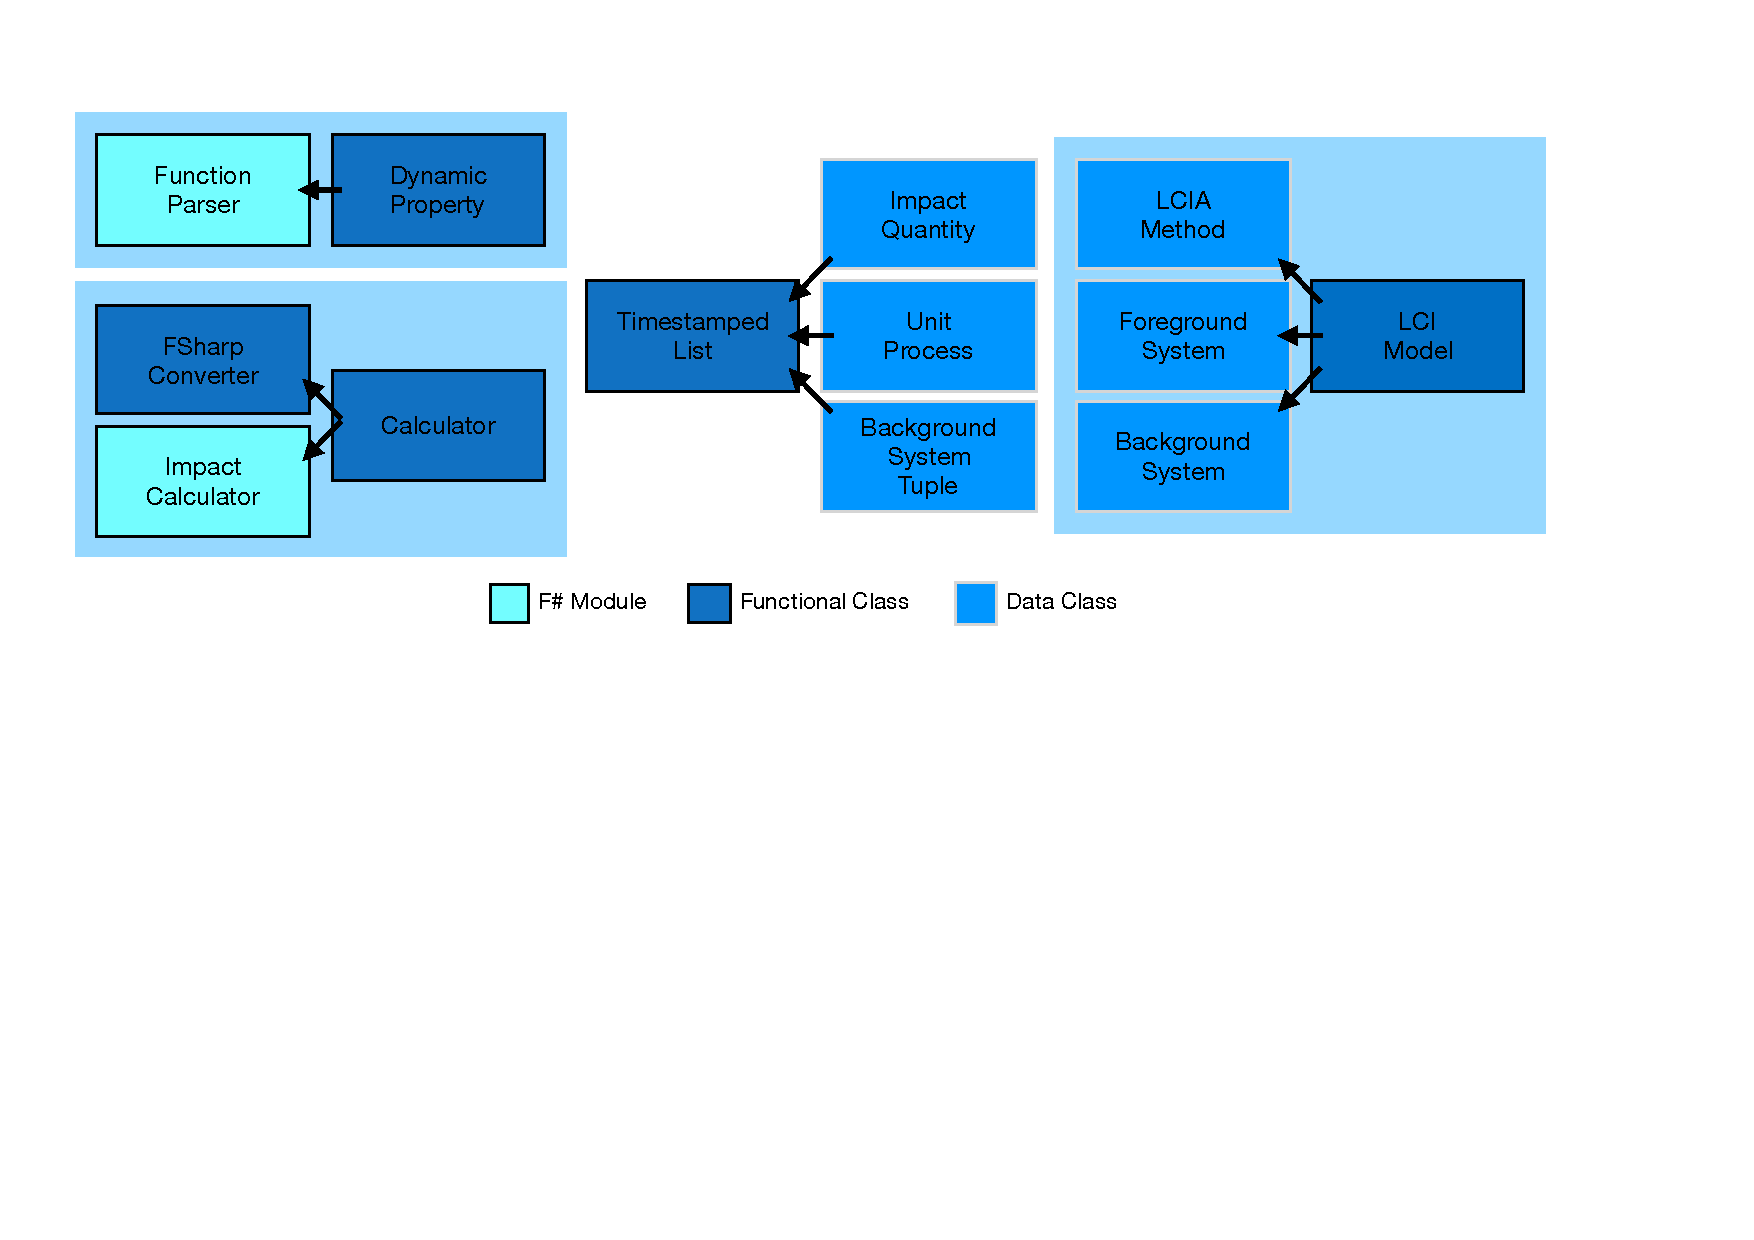
\includegraphics[page=1, width=\linewidth]{.Figures/TestingGroups.pdf}
    \caption{Units and Components which will have unit tests defined, according to the referenced \textit{Development Testing} chapter\cite{SoftwareEngineering}. The titled squares symbolise units and the untitled surrounding squares symbolise components. The arrows symbolise possession and/or dependency.}
    \label{fig:TestingGroups}
\end{figure}

\subsection{Function Parser Module} \label{ssec:Testing-FunctionParserModule}
Recalling from Section \ref{ssec:DynamicProperties}, the function parser module relies on functionality from the \texttt{FParsec} library for operator associativity and hierarchy. The behaviour of this functionality must be checked, as well as its ability to parse the binary functions required to model the function pieces for the dynamic properties.

Tests are written, with focus on:
\begin{itemize}
    \item Failure when unknown syntax is encountered
    \item Constant expressions, with no parameters
    \item Parsing necessary input parameters
    \item Operator associativity for each defined operator
    \item Operator hierarchy
\end{itemize}

The parsed functions are compared with the hierarchy and associativity of operators implemented in F\#, assumed to follow the general rules of mathematics.

The interface for the module contains only the function:

\begin{lstlisting}[language=FSharp]
val Parse: string -> (double -> double -> double)
\end{lstlisting}

which is the entry for the unit tests.

This way, all functionality required by the program is tested and verified.

\subsection{Impact Calculator Module} \label{ssec:Testing-ImpactCalculatorModule}
The module for impact calculations is tested on all steps of the computation according to the algorithm defined in the requirements. 

First, the functions for data handling are tested:

The addition of lists of impact quantities, is tested for expected results as well as expected exceptions when given lists of different lengths or trying to add impact quantities from different categories. 

The scaling of impact quantities by a factor (e.g. the usage of a component), and applying dynamic properties are tested for expected results. 

Next, each type of component is created with example data for the internal data structure. Indicator scores are calculated and compared to the results from the equivalent function in the module. Cases with empty, partially populated and populated components are covered, to test all partitions of input data for the functions.\footnote{Input partitions are defined as the set of input values yielding the same behaviour. When testing components often infinite input values are possible, therefore representatives from each input partition are tested to cover the span of possible inputs. (\cite{SoftwareEngineering} Chapter 8.1.2)}

\vspace{1cm}
The tests for the F\# modules are written and executed in the F\# language, making them independent of the rest of the software implementation. All tests are executed and verified, checking for errors or unwanted behaviours before deploying the compiled \texttt{.dll} file to the main program.

\subsection{Model Handling Classes}

The classes containing critical procedures regarding model interaction consist of; \texttt{LCIModel}, \texttt{DynamicProperty}, and the auxiliary class \texttt{TimestampedList}. 

\texttt{LCIModel} is tested for all methods interacting with the internal data structure. These methods are called from the event handlers in the control classes, and should create/remove components according to the commands of the user.

\texttt{DynamicProperty} contains methods for creating function expressions with corresponding intervals, and methods for composing the piece-wise function based on the individual function expressions and intervals using the function parser module. Finally the class contains a method to execute the correct portion of the piecewise function for the required timestamp. All which is tested, both the class as a unit, but also as a component using the function parser module.

The class \texttt{TimestampedList} is tested for its list of timestamped data, together with methods for accessing and manipulating the list. Together with the \texttt{DynamicProperty} class, they are responsible for providing a snapshot of the LCI model for the given time step.

\subsection{Data Structure Conversion Class}
The class \texttt{FSharpConverer} converts the data structure of interest from the C\# data representation to an F\# data representation, converting from a data structure defined on an interval of timestamps to a snapshot of the data structure for a specific time. This mapping procedure has to be correct for the results to have any credibility, as well as the mapping from the resulting indicator scores back to a C\# data representation before delivering the information to the user.

The class contains methods for converting each of the defined components, and is tested for all input partitions. This means empty, partially populated and populated components are converted, followed by comparing content between the two data representations for the specific timestamp.

The wrapper class \texttt{ImpactCalculator} is not tested as a unit, since the class's methods all follow the same structure, of which each step is tested individually: Convert data, call function from impact calculator module, convert data back and return it. If all conversions and modules are tested, then testing these methods gives no new information. 

\vspace{1cm}
With these tests written and executed for all the specified classes, we can conclude that the \textbf{Unit} and \textbf{Component Testing} steps are satisfied.